\documentclass[twoside,leqno,11pt]{article}
\usepackage{revstat-v2}
\usepackage{amsmath}
\usepackage{enumerate}
\usepackage{amssymb}
\usepackage{graphicx}
\usepackage{hyperref}
\usepackage{color}
\usepackage[utf8]{inputenc}
\usepackage[T1]{fontenc}
\usepackage{pdflscape}
\usepackage{bm}
\usepackage{float}
\usepackage{listings}
\usepackage{xcolor}
\usepackage{color}
\usepackage{caption}
\usepackage{subcaption}

\newcommand{\etn}{{\mbox{\boldmath $\eta$}}} 
\hyphenation{ge-ne-ra-ted  hy-per-geo-me-tric  cha-rac-te-ri-ze}
 
\begin{document}
\thispagestyle{firstpage}

\vspace{-3.2cm}

\noindent
{\footnotesize {\sffamily REVSTAT~~--~~Statistical~~Journal\\[-1pt]
		Volume 0, Number 0, Month 0000,
		000-000}}
% \thepage-\pageref{LastPage}}}   % requires \usepackage{lastpage}

\vspace{1.5cm}
\title{Marshall and Olkin-G and Gamma-G family of distribution: properties and applications
	%\footnote{The opinions expressed in this text are those of the authors and do not necessarily reflect the views of any organization.}
}
\renewcommand{\titleheading}
{MOGG family of distribution: properties and applications}  % --- on odd running heads

\author{\authoraddress{Maria do Carmo S. Lima \href{https://orcid.org/0000-0002-5480-3103}{\includegraphics[scale=0.08]{ORCID-iD_icon-128x128}}} 
	{Department of Statistics,
		Federal University of Pernambuco,\\
        Pernambuco, Recife, Brazil
		\ (maria@de.ufpe.br)}
	\\
	\authoraddress{Gauss M. Cordeiro \href{https://orcid.org/0000-0002-3052-6551}{\includegraphics[scale=0.08]{ORCID-iD_icon-128x128}}}
	{Department of Statistics,
		Federal University of Pernambuco,\\
		Pernambuco, Recife, Brazil
		\ (gauss@de.ufpe.br)}
	\\
	\authoraddress{Pedro Rafael D. Marinho \href{https://orcid.org/0000-0003-1591-8300}{\includegraphics[scale=0.08]{ORCID-iD_icon-128x128}}
	\correspondingauthor}
	{Department of Statistics,
		Federal University of Paraíba,\\
		Paraíba, João Pessoa, Brazil
		\ (pedro.rafael.marinho@gmail.com)}
}
\renewcommand{\authorheading}
{Maria do Carmo S. Lima, Gauss M. Cordeiro and Pedro Rafael D. Marinho, }  % --- on even running heads

%\vspace{0.3in}
%First Version: 27 July 2010\\
%\vspace{0.1in}
%This Version: 27 January 2011\\

%-------------------------------------------------------------------------------
% Just asking LaTeX to effectively do the title...
%-------------------------------------------------------------------------------
\maketitle
%-------------------------------------------------------------------------------
% Just asking LaTeX to numerate lines...
%-------------------------------------------------------------------------------
\setpagewiselinenumbers
\modulolinenumbers[1]
\linenumbers
%%%%%%%%%%%%%%%%%%%%%%%%%% alteracao: Datas %%%%%%%%%%%%%%%%%%%%%%%%%%%%%%%%%%
\noindent
~~~~{\small{\sffamily Received:} December 2020 ~~~~~~{\sffamily Revised:} May 2022 ~~~~~~{\sffamily Accepted:} Month 0000}
%%%%%%%%%%%%%%%%%%%%%%%%%% alteracao %%%%%%%%%%%%%%%%%%%%%%%%%%%%%%%%%%

%-------------------------------------------------------------------------------
% Abstract of the article...
%-------------------------------------------------------------------------------
\begin{abstract}
This article introduces a new family by combining the Marshall and Olkin-G and Gamma-G classes. The family has only two
extra shape parameters and can be a better model  than other existing classes of distributions. Simulations are performed to verify the
consistency of the estimators. Its flexibility is shown using two real data sets.
\end{abstract}

%-------------------------------------------------------------------------------
% Keywords...
%-------------------------------------------------------------------------------
\begin{keywords}
 Distribution family;  mathematical properties; simulations; applications.
\end{keywords}

%-------------------------------------------------------------------------------
% AMS classifications...
%-------------------------------------------------------------------------------
\begin{ams}
	60E05, 62E10, 62E15.
\end{ams}

\section{INTRODUCTION}

The mechanism by adding shape parameters to a baseline distribution has
proved to be useful to make the generated distributions more flexible especially for studying tail
properties than existing distributions and for improving their goodness-of-fit statistics
to the data under study. Many special distributions in these families are discussed by Tahir
and Nadarajah (2015).

Let $G(x)$ be the cumulative distribution function (CDF) of a
baseline distribution and $g(x)=dG(x)/dx$ be the corresponding  probability density function (PDF) depending on a
parameter vector $\eta$. A generalized family are presented
with two additional shape parameters by transforming the CDF $G(x)$
according to two sequential important gene\-rators. These families are important for modeling data
in several engineering areas. 


The CDF of the Marshall and Olkin's (1997) ($\text{MO-G}$) family (for $\theta>0$) is
\begin{equation}\label{CDF_MO}
F_{\text{MO-G}}(x)=\frac{G(x)}{\theta+(1-\theta)G(x)}=\frac{G(x)}{1-(1-\theta)[1-G(x)]},\quad x \in \mathbb{R}.
\end{equation}

The density function corresponding to (\ref{CDF_MO}) has the form
\begin{equation}\label{densityMO}
f_{\text{MO-G}}(x)=\frac{\theta\, g(x)}{[\theta+(1-\theta)G(x)]^{2}}.
\end{equation}

For $\theta=1$, $f_{\text{MO-G}}(x)$ is equal to $g(x)$. 
Equation \eqref{densityMO} represents the PDF of the minimum of $n$ iid random variables having density $g(x)$, say $T_1,\cdots,T_N$, 
where $N$ has a geometric distribution with probability parameters $\theta$ and $\theta^{-1}$ if $0<\theta<1$ and $\theta>1$, 
respectively.

Tahir and Nadarajah (2015, Table 2) presented thirty distributions
belonging to this family. It is easily generated from the baseline quantile function (QF) by
$Q_{\text{MO-G}}(u)=Q_{G}\left(\theta u / \left[\theta u+1-u\right]\right)$ for $u\in(0,1)$.

Marshall and Olkin considered the exponential and Weibull distributions for the baseline G and derived some
structural properties of the generated distributions. The special case that G is an exponential distribution
refers to a two-parameter competitive model to the Weibull and gamma distributions.

The CDF of the gamma-G ($\Gamma$-G) family (Zografos and Balakrishnan, 2009) is
\begin{eqnarray}\label{CDF_Ga}
F_{\Gamma\text{-G}}(x)=\gamma_1\left( a, -\log \left[1-G(x)\right]\right), \quad x \in \mathbb{R},
\end{eqnarray}
where $a>0$ is an extra shape parameter,  $\gamma_1(a,z)= \gamma(a,z)/\Gamma(a)$ is the incomplete gamma function ratio
and $\gamma(a,z)=\int_0^{z} t^{a-1}\,\rm{e}^{-t}dt$.

Then, the PDF of the $\Gamma$-G family can be expressed as
\begin{eqnarray}\label{PDF_Ga}
\displaystyle
f_{\Gamma\text{-G}}(x)=\frac{\displaystyle 1}{\displaystyle \Gamma(a)} \left\{ -\log[1-G(x)] \right\}^{a-1}\, g(x).
\end{eqnarray}

Each new $\Gamma$-G distribution follows from a given baseline G.
For $a=1$, the $\Gamma$-G family reduces to G.
If $Z$ is a gamma random variable with unit scale
parameter and shape parameter $a>0$, then $W=Q_G(1-\rm{e}^{-Z})$ has density (\ref{PDF_Ga}). So,
the $\Gamma$-G distribution is easily generated from the gamma distribution and the QF of G.

The remaining of the paper is addressed as follows. Section \ref{sec:MOGaG} introduces the {\it Marshall and Olkin-Gamma-G} (MOGa-G)
family and presents some special models. The maximum likelihood estimates (MLEs) of the parameters of the new family is addressed
in Section \ref{estimation}. Some simulations ate performed in Section \ref{sec:simulation} to estimate the biases of the MLEs. Two
empirical applications illustrate the potentiality of the proposed family in Section \ref{applications}. A variety of theoretical properties are derived
in Section \ref{properties}. Some conclusions remarks are offered in Section \ref{conclusions}.

\section{THE NEW FAMILY}\label{sec:MOGaG}

By combining Equations (\ref{CDF_MO}) and (\ref{CDF_Ga}), the CDF of the random variable $X\sim$MOGa-G
representing the new family is defined by
\begin{equation}\label{CDF_MO-Gamma-G}
F_{X}(x)=\frac{\gamma_1\left( a, -\log \left[1-G(x)\right]\right)}{\theta+(1-\theta)\gamma_1\left( a, -\log \left[1-G(x)\right]\right)},\quad x \in \mathbb{R}.
\end{equation}

By differentiating (\ref{CDF_MO-Gamma-G}), the PDF of $X$ follows as
\begin{equation}\label{PDF_MO-Gamma-G}
f_{X}(x)=\frac{\theta  \left\{ -\log[1-G(x)] \right\}^{a-1}\, g(x)}{\Gamma(a)\,\left\{\theta+(1-\theta)\gamma_1\left( a, -\log \left[1-G(x)\right]\right)\right\}^{2}}.
\end{equation}

The density (\ref{PDF_MO-Gamma-G}) can be interpreted from a sequence of $N$ iid random variables, say $Z_1,\cdots,Z_N$,
each one having a gamma density with unit scale parameter and shape parameter $a>0$, assuming that $N$ (is not fixed) has a geometric 
distribution with probabilities $\theta$ and $\theta^{-1}$ for $0<\theta<1$ and $\theta>1$,
respectively. By transforming the $Z_i$'s via the baseline QF by $W_i=Q_G(1-\rm{e}^{-Z_i})$
(for $i-1,\ldots,N$), Equation \eqref{densityMO} is defines the PDF of the minimum $W_1,\cdots,W_n$. 
Making this double composition of the two generators, the proposed family absorbs the impacts of two different flexibilities 
on applications. 


Table 1 provides some special cases of (\ref{PDF_MO-Gamma-G}), where
$\Phi(x)$ and $\phi(x)$ are the CDF and PDF of the standard normal distribution. The density and hazard functions
of the Marshall-Olkin-$\Gamma$-Weibull (MOGa-W) defined by $h(x) = f(x)/(1-F(x))$ are displayed in Figure \ref{formas}, which provide
more flexibility for these functions in relation to the baseline ones.

\vspace{0.6cm}

%\begin{figure}[H]
%\begin{center}
%\includegraphics[scale =  0.39]{pdf-hazard.pdf}
%\caption{(A) MOGa-W density. (B) MOGa-W hazard.\label{formas}}
%\end{center}
%\end{figure}

\begin{figure}
	\centering
	\begin{subfigure}[b]{0.49\textwidth}
		\centering
		\includegraphics[width=\textwidth]{pdf_function.pdf}
		\caption{MOGa-W density function.}
		\label{fig:pdf}
	\end{subfigure}
	\hfill
	\begin{subfigure}[b]{0.49\textwidth}
		\centering
		\includegraphics[width=\textwidth]{hazard_function.pdf}
		\caption{MOGa-W hazard function.}
		\label{fig:hazard}
	\end{subfigure}
\caption{MOGa-W density function and  MOGa-W hazard function with G following the Weibull distribution.}
\label{formas}
\end{figure}

\vspace{0.6cm}

The CDF \eqref{CDF_MO-Gamma-G} can be easily inverted to calculate the QF of the MOGa-G distribution,
say $x=Q_{X}(u)=F_X^{-1}(u)$ for $u \in (0,1)$, in terms of the Q$_F$ of the baseline distribution G, $Q_G(\cdot)$. The inverse of
$F_{X}(x)=u$, where $u$ is a uniform number in $(0,1)$ is easily obtained. By combining the inverses
of Equations (\ref{CDF_MO})and \eqref{CDF_MO-Gamma-G}, $F_{X}(x)=u$ leads to
$z=z(u)=\theta u/[1-(1-\theta)u]$ and $\gamma_{1}\left(a, -\log[1-G(x)]\right)=z(u)$.
Then, the QF of $X$ can be expressed as
$$x=Q_G\left(v(u)\right),$$
where
$$v(u)=1-\exp\left[-\gamma_1^{-1}\big(a,z(u)\big)\right],$$
and $\gamma_1^{-1}(a,w)=Q^{-1}(a,1-w)$ is the inverse function of $\gamma_1(a,w)$. Some formulae for
$Q^{-1}(a,1-w)$ are given in \url{http:// functions.wolfram.com/ GammaBetaErf/ InverseGammaRegularized/}.

\begin{landscape}
	\begin{table}[htbp]\label{tabspecial1}
		\caption{Special Distributions in the  MOGa-G family.}
		\centering
\scalebox{0.7}{	
		\begin{tabular}{l|l|l}
			\hline
			\textbf{Distribution} & \textbf{Baseline CDF} & \textbf{Generated PDF}  \\
			\hline
			{} & {} & {} \\
			\textbf{Normal} &  $G(x)=\Phi(x)$ & $f_{X}(x)=\frac{\theta  \left\{ -\log[1-\Phi(x)] \right\}^{a-1}\, \phi(x)}{\Gamma(a)\,\left\{\theta+(1-\theta)\gamma_1\left( a, -\log \left[1-\Phi(x)\right]\right)\right\}^{2}}$ \\
			{} & {} & {} \\
			\hline
			{} & {} & {} \\
			\textbf{Logistic} &  $G(x)=\frac{1}{1+\rm{e}^{-x}}$ & $f_{X}(x)=\frac{\theta\,\rm{e}^{-x}\, \left\{ -\log[1-(1+\rm{e}^{-x})^{-1}] \right\}^{a-1}}{\Gamma(a)\,(1+\rm{e}^{-x})^{2}\,\left\{\theta+(1-\theta)\gamma_1\left( a, -\log \left[1-(1+\rm{e}^{-x})^{-1}\right]\right)\right\}^{2}}$\\
			{} & {} & {} \\
			\hline
			\textbf{Gumbel} &  $G(x)=1-\exp(-\rm{e}^x)$ & $f_{X}(x)=\frac{\theta \, \exp(a \,x-  \rm{e}^x)}{\Gamma(a)\,\left\{\theta+(1-\theta)\gamma_1\left(a, \rm{e}^{x}\right)\right\}^{2}}$ \\
			{} & {} & {} \\
			\hline
			{} & {} & {} \\
			\textbf{Log-Normal} &  $G(x)=\Phi(\log x)$ & $f_{X}(x)=\frac{\theta\,\phi(\log x)\,  \left\{ -\log[1-\Phi(\log x)] \right\}^{a-1}}{\Gamma(a)\,x\,\left\{\theta+(1-\theta)\gamma_1\left( a, -\log \left[1-\Phi(\log x)\right]\right)\right\}^{2}}$ \\
			{} & {} & {} \\
			\hline
			{} & {} & {} \\
			\textbf{Exponential} &  $G(x)=1-\exp(-\lambda x),\,\lambda>0$ & $f_{X}(x)=\frac{\theta\,\lambda^{a}\,x^{(a-1)}\, }{\Gamma(a)\,\left\{\theta+(1-\theta)\gamma_1\left(a,\lambda x\right)\right\}^{2}}$ \\
			{} & {} & {} \\
			\hline
			{} & {} & {} \\
			\textbf{Weibull} &  $G(x)=1-\exp(-(\lambda x)^\gamma),\,\lambda,\gamma>0$ & $f_X(x)=\frac{\theta\,\gamma\lambda^{a\,\gamma}x^{a\,\gamma-1}\exp\{-(\lambda\,\gamma)^\gamma\}}{\Gamma (a)\{\theta+(1-\theta)\gamma_1[a,(\lambda\,x)^\gamma]\}^2}$ \\
			{} & {} & {} \\
			\hline
			{} & {} & {} \\
			\textbf{Gamma} &  $G(x)=\gamma_1(\alpha,\beta x),\,\alpha,\,\beta>0$ & $f_{X}(x)=\frac{\theta\,\beta^{\alpha}\,x^{\alpha-1}\,\rm{e}^{-\beta x}\,\left\{ -\log[1-\gamma_1(\alpha,\beta x)] \right\}^{a-1}}{\Gamma(a)\,\left\{\theta+(1-\theta)\gamma_1\left( a, -\log \left[1-\gamma_1(\alpha,\beta x)\right]\right)\right\}^{2}}$ \\
			{} & {} & {} \\                                                                                                                                                                          \hline
			\textbf{Pareto} &  $G(x)=1-\frac{1}{(1+x)^\nu},\,\nu>0$ & $f_{X}(x)=\frac{\theta \, \rm{e}^{-x}\, \left[\nu\log(1+x)\right]^{a-1}\, g(x)}{\Gamma(a)\,(1+\rm{e}^{-x})^2\,\left\{\theta+(1-\theta)\gamma_1\left( a, \nu\log[1+x]\right)\right\}^{2}}$\\
			{} & {} & {} \\
			\hline
			\textbf{Dagum} & $G(x) = \Big[1 + \Big(\frac{x}{\beta}\Big) ^ {-\alpha}\Big] ^ {-p},\,\, \alpha, \beta, p > 0$ & $f_X(x) = \frac{\theta  \left\{ -\log[1-G(x)] \right\}^{a-1}\, g(x)}{\Gamma(a)\{\theta + (1 - \theta)\gamma_1[a, -\log   (1-((x/\beta)^{-\alpha}+1)^{-p})]\}}$ \\
			\hline
		\end{tabular} }
	\end{table}
\end{landscape}

\section{ESTIMATION}\label{estimation}

The  MOGa-G family can be  fitted to real data using the {\bf AdequacyModel} package, {\color{red}Marinho et al. (2019)}, in the {\sf R} software.
This packa\-ge does not require to define the log-likelihood function and it computes the MLEs, their standard errors (SEs)
and the formal statistics defined in Section \ref{applications}. It is necessary to provide the
PDF and CDF of the distribution to be fitted to a data set.

For example, if $x_i$ is one observation from (\ref{PDF_MO-Gamma-G}) and $\etn$ is a $q$-parameter vector specifying $G(\cdot)$,
the log-likelihood function for $\boldsymbol{\theta}^\top=(a,\theta,\etn^\top)$ from $n$ observations is
\begin{align}\label{loglik}
\ell (\boldsymbol{\theta})=&\,n\log (\theta)+n\log(\gamma)+n\, a\, \gamma \log(\lambda)+(a\gamma-1)\sum_{i=1}^n{\log(x_i)}-\lambda^\gamma\sum_{i=1}^n{\log(x_i)}\nonumber \\ &
-n\log[\Gamma(a)]-2\sum_{i=1}^n{\log\{\theta+(1-\theta)\gamma_1[a,(\lambda\,x_i)^\gamma]\}}.
\end{align}

Due to the impossibility of obtaining the MLEs in closed form, numerical methods to obtain the estimates that maximize $ \ell (\cdot) $ are necessary. Several programming languages and statistical software distributes functions and routines that make it easy to obtain numerical estimates by various interactive methods. In practice, obtaining the MLEs for the parameters that index a probability distribution are commonly obtained in this way, since the Newton and quasi-Newton methods produce satisfactory results under reasonable conditions of the object function, that is, when they do not impose conditions that disturb the convergence of the algorithms.

To obtain the MLEs, the package {\bf AdequacyModel} of the programming language {\sf R} was used, see R Core Team (2020). This library, created and maintained by one of the authors of this paper, is widely cited by several papers in the field of statistics and serves as a basis for other library implementations available on the Comprehensive R Archive Network - CRAN.  With it, in particular using the goodness.fit function, it is possible to provide an implementation {\sf R} of (\ref {PDF_MO-Gamma-G}), being in charge of this function, obtain $\ell(\cdot)$  by returning several measures of fit adequacy as well as the MLEs. Further details regarding this package can be obtained from Marinho et al. (2019).


\section{SIMULATIONS}\label{sec:simulation}

{\color{red}Due to the probable absence of MLEs in closed-form for distributions belonging to the MOGa-G family, it is necessary to examine the precision of the estimates calculated numerically. 

For doing that, the biases of the estimators of the parameters of the
MOGa-Dagum($\theta$, $a$, $\alpha$, $\beta$, $p$) and  MOGa-Weibull($\theta$, $a$, $\lambda$, $\gamma$) distribution are determined, where $G\sim \mathrm {Dagum} (\alpha, \beta, p)$ and  $\mathrm {Weibull} (\gamma, \lambda)$ are the baselines distributions, respectively. All parameters are taken equal to one for different sample sizes reported in the Tables \ref{tab:bias1} and \ref{tab:bias2}. 

The Tables \ref{tab:bias1} and \ref{tab:bias2} indicate that this method behaves well when the sample size increases. This is theoretically expected. However, in practice, difficulties can be faced in other families of distributions due to the flatness of the log-likelihood function.

All simulations can be reproduced using the script in \url{https://github.com/prdm0/MOGG}. The simulations are parallelized and able to use all threads available by a multicore processor, thus making them more computationally efficient and consequently requiring less time to complete. 

The simulations are performed on a computer with an Intel(R) Core(TM) i5-9500 CPU processor with 6 threads working at a maximum frequency of 3.00GHz, requiring, on these hardware, a time of 15.4828 hours to perform all simulations, 7.7414 hours for the MOGa-Dagum($\theta$, $a$, $\alpha$, $\beta$, $p$) distribution and 4.9688 hours for the MOGa-Weibull($\theta$, $a$, $\lambda$, $\gamma$) distribution. The  Tables \ref{tab:bias1} and  \ref{tab:bias2} reveal that the average biases of the MLEs could be very reduced only for $n> 2,000$.}

To generate observations from the random variable $X$ with density $f$, the well-known Acceptance-Rejection Algorithm for continuous random variables, which is very useful when the quantile function involves complex functions that can lead to some numerical inaccuracies. For doing this, another random variable $Y$ is chosen such that it can generate observations from a PDF $h$ with the same support as $f$. Then, the acceptance and rejection algorithm is defined by the following steps:
\begin{enumerate}
	\item Generate an outcome $y$ from $Y$;
	\item Generate an observation $u$ from a random variable $U\sim \mathcal{U}(0,1)$;
	\item If $u < \frac{f(y)}{c\, g(y)}$, where $c$ is a real constant, accept $x=y$; otherwise reject $y$ as an outcome from $X$ and return to 1.
\end{enumerate}

The constant $c$ must be chosen in such a way that $\frac{f(y)}{c \,g (y)}\leq 1 $. 
Thus, to minimize the computational cost of generating observations from $X$ through the generated observations from $Y$, $c$ is chosen 
as the lowest possible value to maximize the likelihood of acceptance. Further details of this method can be found in Rizzo (2019).

\begin{table}[H]
	\centering
	\caption{\textcolor{red}{Mean biases of the MLEs of the MOGa-Dagum($\theta$, $a$, $\alpha$, $\beta$, $p$) distribution obtained by the BFGS method calculated from the Monte-Carlo simulation.}}\label{tab:bias1}
	\begin{tabular}{rrrrrrr}
		\hline
		$n$ & $B(\hat{\theta})$ & $B(\hat{a})$ & $B(\hat{\alpha})$ & $B(\hat{\beta})$ & $B(\hat{p})$ & Time (mins)\\
		\hline
10 & 0.2213 & 2.1944 & 2.6971 & 1.5803 & 1.3190 & 0.6960 \\ 
20 & 0.4240 & 2.4793 & 1.5591 & 1.8083 & 0.7414 & 0.9819 \\ 
60 & 0.7458 & 2.2661 & 0.5598 & 1.8495 & 0.2812 & 1.9417 \\ 
100 & 0.6194 & 1.9438 & 0.3312 & 1.6142 & 0.2935 & 2.7208 \\ 
200 & 0.3950 & 1.4262 & 0.1856 & 1.1556 & 0.3611 & 4.4534 \\ 
400 & 0.2077 & 0.9599 & 0.1082 & 0.6157 & 0.4076 & 7.4698 \\ 
600 & 0.1200 & 0.7213 & 0.0767 & 0.4024 & 0.3572 & 9.4975 \\ 
1000 & 0.0629 & 0.4791 & 0.0503 & 0.2123 & 0.2584 & 12.4221 \\ 
2000 & 0.0362 & 0.2958 & 0.0298 & 0.1145 & 0.1878 & 20.7251 \\ 
5000 & -0.0040 & 0.1325 & 0.0159 & 0.0144 & 0.0167 & 28.3380 \\ 
10000 & -0.0133 & 0.0815 & 0.0096 & 0.0081 & 0.0039 & 50.9298 \\ 
20000 & -0.0111 & 0.0349 & 0.0037 & 0.0006 & -0.0109 & 68.6320 \\ 
30000 & -0.0036 & 0.0191 & 0.0006 & -0.0041 & -0.0034 & 97.3046 \\ 
50000 & -0.0057 & 0.0129 & 0.0016 & 0.0015 & -0.0026 & 158.3737 \\ 
		\hline
	\end{tabular}
\end{table}

\begin{table}[H]
	\centering
	\caption{\textcolor{red}{Mean biases of the MLEs of the MOGa-Weibull($\theta$, $a$, $\lambda$, $\gamma$) distribution obtained by the BFGS method calculated from the Monte-Carlo simulation.}}\label{tab:bias2}
	\begin{tabular}{rrrrrr}
		\hline
		$n$ & $B(\hat{\theta})$ & $B(\hat{a})$ & $B(\hat{\lambda})$ & $B(\hat{\gamma})$ & Time (mins)\\
		\hline
		10 & 0.0818 & 0.1362 & 4.9274 & 1.2407 & 0.6716 \\ 
		20 & 0.3404 & -0.0177 & 3.4160 & 1.4117 & 0.8077 \\ 
		60 & 0.7037 & -0.0677 & 1.8806 & 1.3385 & 1.1773 \\ 
		100 & 0.6698 & -0.0535 & 1.3684 & 1.1796 & 1.2643 \\ 
		200 & 0.5371 & -0.0299 & 0.8265 & 0.9110 & 1.7886 \\ 
		400 & 0.3371 & -0.0047 & 0.4205 & 0.5967 & 2.8386 \\ 
		600 & 0.2457 & 0.0076 & 0.2685 & 0.4306 & 3.6867 \\ 
		1000 & 0.1476 & 0.0093 & 0.1553 & 0.2818 & 5.0944 \\ 
		2000 & 0.0731 & 0.0035 & 0.0758 & 0.1530 & 8.8577 \\ 
		5000 & 0.0264 & 0.0007 & 0.0283 & 0.0618 & 15.8586 \\ 
		10000 & 0.0128 & -0.0007 & 0.0142 & 0.0318 & 29.8629 \\ 
		20000 & 0.0053 & -0.0012 & 0.0071 & 0.0160 & 48.7417 \\ 
		30000 & 0.0023 & -0.0014 & 0.0053 & 0.0119 & 64.7387 \\ 
		50000 & 0.0023 & -0.0004 & 0.0028 & 0.0063 & 112.7422 \\ 
		\hline
\end{tabular}
\end{table}


\section{APPLICATIONS}\label{applications}

Consider the Weibull baseline. Two applications are provided to compare the new generated model with seven extended Weibull
distributions, namely the beta-Weibull ($\beta$-W) (Famoye {\it et al.}, 2005), Kumaraswamy Weibull (Kw-W) (Cordeiro and Nadarajah, 2010),
Marshall-Olkin Weibull (MO-W) (Ahmed {\it et al.}, 2017), Marshall-Olkin Extended Weibull (MOE-W) (Cordeiro {\it et al.}, 2019),
exponentiated Weibull (exp-W) (Mudholkar and Srivastava, 1993), gamma Weibull ($\Gamma$-W) Cordeiro {\it et al.}, 2016) and exponentiated
generalized Weibull (EG-W) (Oguntunde {\it et al.}, 2015) (with $a=1$). Some of these distributions are widely used in practice.

The log-likelihood for the Marshall-Olkin-Gamma-Weibull (MOGa-W) from one observation is
\begin{align}
\ell (\boldsymbol{\theta})=& \log (\theta)+\log (\gamma)+(a\,\gamma)\log (\lambda)+(a\,\gamma-1)\log(x)-(\gamma\, x)^\gamma-\log[\Gamma(a)]\nonumber \\ &-2\log\{\theta+(1-\theta)\gamma_1[a,(\lambda\,x)^\gamma]\},
\end{align}
where $\boldsymbol{\theta}=(a,\theta,\lambda,\gamma)^\top$. The components of the score function are

\begin{equation*}
U_{a}(\boldsymbol{\theta})=\gamma  \log (\lambda )+\gamma  \log (x)-\psi ^{(0)}(a)-\frac{2\left\{(1-\theta ) A-(1-\theta ) \psi ^{(0)}(a) \gamma_1 \left[a,(x \lambda
   )^{\gamma }\right]\right\}}{\theta\,\Gamma(a)+(1-\theta)\gamma_1\left[a,(x \lambda
   )^{\gamma }\right]},
\end{equation*}

\begin{equation*}
U_{\theta}(\boldsymbol{\theta})=\frac{1}{\theta}-\frac{2\left\{\Gamma(a)-\gamma_1\left[a,(\lambda\,x)^\gamma\right]\right\}}{\theta\,\Gamma(a)+(1-\theta)\gamma_1\left[a,(\lambda\,x)^\gamma\right]},
\end{equation*}

\begin{equation*}
U_{\lambda}(\boldsymbol{\theta})=\frac{\gamma }{\lambda }\left[a-(\lambda\,x)^\gamma\right]+\frac{2 \gamma \,\lambda^{-1}(\lambda\,x)^{a\,\gamma} (1-\theta )\exp\{-(\lambda\,x)^\gamma\} }{\theta \,\Gamma(a)+(1-\theta )
   \gamma_1 \left[a,(x \lambda )^{\gamma }\right]}
\end{equation*}
and
\begin{equation*}		
U_{\gamma}\boldsymbol{\theta}=\frac{1}{\gamma }+a \log (\lambda )+a \log (x)-(\lambda  x)^{\gamma } \log
   (\lambda  x)+\frac{2 (1-\theta )(\lambda
   x)^{\gamma\,a } \log (\lambda  x)\exp\{-(\lambda  x)^{\gamma }\}  }{\theta \,\Gamma(a)+(1-\theta )
   \gamma_1 \left[a,(x \lambda )^{\gamma }\right]},
\end{equation*}
where
\begin{align*}
A=G_{2,3}^{3,0}\left[(x \lambda )^{\gamma }\Big{|}
\begin{array}{c}
 1,1 \\
 0,0,a \\
\end{array}
\right]+\log \left[(\lambda  x)^{\gamma }\right] \gamma_1 \left[a,(x \lambda )^{\gamma
   }\right],
\end{align*}
$\psi^{(n)}(x)$ is the $n$-th derivative of the digamma function,
\begin{eqnarray*}
A=\psi^{(0)}(a) - \log\left[(\lambda x)^{\gamma}\right]-G^{3,0}_{2,3}\,\left((\lambda x)^{\gamma} \Big{|}	\stackrel{1,1}{0,0,a}\right),
\end{eqnarray*}
and $G^{m,n}_{p,q}\,\left(z \Big{|}	\stackrel{a_{1},\ldots,a_{p}}{b_{1},\ldots,b_{q}}\right)$ is the Meijer G function.

The {\bf AdequacyModel} is used to fit the distributions cited before to two real data sets. The SANN method, which is a
variant of simulated annealing (Belisle, 1992), is considered. The distributions are compared via the Anderson
Darling (A$^{*}$) and Cram\'er Von Mises (W$^{*}$) statistics reported in the {\tt goodness.fit} function.

For the first data set, a modification of the ``FoodExpenditure'' data from the {\bf betareg} package  is considered, which refers
to the proportions of income spent on food for a random sample of 38 households in a large US city (according to the package information).
Here, the household expenditures for food are considered and is given by
\begin{eqnarray*}
data = FoodExpenditure_{food} / \#(FoodExpenditure_{food}),
\end{eqnarray*}
where $FoodExpenditure_{food}$ is the random variable corresponding to the household expenditures for food and $\#(\cdot)$ indicates the number of
observations on this variable. \textcolor{red}{Some descriptive statistics are displayed from Table \ref{tabds}. }


\begin{table}[!htb] 
\scriptsize
\center
\caption{Descriptive statistics for the first data}
\label{tabds}
\begin{tabular}{ ccccccccc}
\hline\noalign{\smallskip}
   Min. & 1st Qu.&  Median&    Mean& 3rd  Qu.&    Max. & sd &skewness & kurtosis\\
   \hline
 0.1956  &0.2913 & 0.3903 & 0.4198 & 0.5027 & 0.7626 & 0.148009 & 0.5250021 & -0.4440273\\
\hline
\end{tabular}
\end{table}

\textcolor{red}{The minimum value in the table above refers to a family that has 3 people and with a family income of 39,.151US, which does not represent the lowest family income in the data set in question, as expected, occupying only the fifth position among those with the lowest income. The maximum value represents a family with a family income of 69,.929US and with 6 people, the second largest number among the number of people per family in the group in question. Furthermore, we can observe that the considered dataset presents positive asymmetry and negative kurtosis. Additionally, the standard deviation (sd) is relatively low.
Figure \ref{ttt} of the data set referring to the first application indicates the decreasing form for the failure rate function. Therefore, these plots indicate the appropriateness of the MOGa-W distribution to fit these data, since the new model can present this form of the hrf, as showed in Figure \ref{fig:hazard}.
}

\begin{figure}[H]
\begin{center}
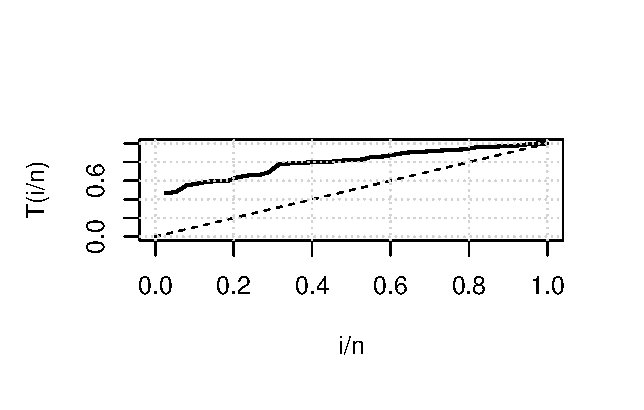
\includegraphics[scale =  1]{ttt1.eps}
\caption{TTT plot for the fisrt data.\label{ttt}}
\end{center}
\end{figure}


The MLEs and their standard errors (SEs) (in parentheses) are listed in Table \ref{tab-ex1}.
The statistics  W$^{*}$ and A$^{*}$ are also given in this table. The results indicate that the proposed model has better performance than the other
seven fitted models.


\begin{table}[!htb]
\scriptsize
\center
\caption{  \small Application 1}
\label{tab-ex1}
\begin{tabular}{lcccccc}
\hline\noalign{\smallskip}
Model & $a$ & $\theta$ & $\lambda$ & $\gamma$ &  $W^*$ & $A^*$   \\
\hline \\
 & & & & &  \\
MOGa-W$(a,\theta,\lambda,\gamma)$    &  0.926134 & 1.379664 & 33.323073 & 25.398809 & 0.0339 &  0.2376 \\                            &    (0.02626926) & (0.22381086) & (0.28530971) & (0.08259864)  & & \\

 & & & & &  \\
$\beta-$W$(a,\theta,\lambda,\gamma)$ &   9.92882 &  0.1700880 & 9.759469 & 1.530541  & 0.043567 & 0.2594618\\
                                    &    (0.02908181) & (0.02049663) & ($<$0.0001) & ($<$0.0001)  && \\
                                                                                & & & & &  \\
KW-W$(a,\theta,\lambda,\gamma)$ &    0.04987575 & 99.99989793 &  1.07602954 & 23.40287099 & 1.330915 & 6.742609\\
                                       &    (0.008090352) & (16.225905058) &  (0.003156126) &  (0.014646102) && \\																						 & & & & &  \\
                                       MOE-W$(a,\theta,\lambda,\gamma)$  &  0.1366666 & 2.020436 & 62.72201 & 4.2956659  &0.03541554 & 0.2579222 \\
 & (0.1599182) & ($<$0.0001) &($<$0.0001) & (0.7365535)    &  & \\
                                                                              & & & & &  \\
EGW$(a,b,\lambda,\gamma)$    &  5.6189861421 &  6.1833138579 &  1.2870816760  & 1.3798562942  &  0.03715255 & 0.2518879 \\
& (0.0028147823) & (0.0009807091) & (0.1159810838) & (0.1480747352)    &  & \\
                                                           & & & & &  \\                                                           MO-W$(a,\lambda,\gamma)$  & 0.15920715  & - &  1.58609458  & 4.26713785  &  0.03456333   & 0.257339\\
&    (0.07170351) & (-) & (0.13353716) & (0.16650667)  &  & \\

 & & & & &  \\
exp-W$(a,\lambda,\gamma)$   &    6.1102948   & - &   4.4680469 &  1.3858740 &   0.03726684   & 0.2523749 \\
&   (0.4222173) & (-) & (0.3175876) & (0.1677722)   &  & \\

 & & & & &  \\
$\gamma$-W$(a,\lambda,\gamma)$    & 5.751546  & - &  10.0000 & 1.208773&  0.0879 & 0.6599  \\
&  (0.0015006)&  (-)&  (0.0001163185) &(0.00822782)    &  & \\

 & & & & &  \\





%GammaBS$(a,b,\alpha)$     &  1.2354 & 40.4438 &  0.1379 &       & 0.4931 &   2.7656 &  0.3725 & $1.765x10^{-12}$\\
                          %&  ( 0.0025)& ( 14.6913)& (0.0446) &      & &&  && \\
                                                     \hline
\end{tabular}
\end{table}



As a second application, consider a data set collected in a pilot study about hypertension in the Dominican Republic
in 1997. The observations are the systolic blood pressure of persons who came to medical clinics in
several villages for a variety of complaints. 
\textcolor{red}{ The data set in question has the following observations} 
         150,
         120,
         120,
         180,
         138,
         115,
         130,
         150,
         200,
         120,
         190,
         90,
         130,
         120,
         200,
         140,
         110,
         134,
         160,
         140,
         105,
         126,
         129,
         120,
         100,
         130,
         118,
         144,
         180,
         138,
         110,
         140,
         120,
         118,
         110,
         110,
         130,
         140,
         130,
         165,
         180,
         130,
         140,
         112,
         130,
         158,
         112,
         150,
         140,
         142,
         110,
         140,
         130,
         132,
         140,
         140,
         122,
         128,
         90,
         118,
         120,
         110,
         122,
         200,
         110,
         140,
         150,
         120,
         150,
         120,
         164,
         122,
         112,
         130,
         140,
         102,
         122,
         130,
         102,
         130,
         122,
         200,
         140,
         180,
         124,
         110,
         124,
         90,
         120,
         159,
         142,
         140,
         118,
         122,
         108,
         170,
         120,
         140,
         100,
         118,
         110,
         114,
         150,
         160,
         140,
         190,
         118,
         120,
         150,
         120,
         200,
         150,
         168,
         110,
         142,
         150,
         160,
         142,
         160,
         150,
         110,
         128,
         122,
         150,
         140,
         122,
         120,
         130,
         100,
         130,
         150,
         130,
         100,
         120,
         105,
         100,
         150,
         196,
         130,
         110,
         140,
         122,
         110,
         164,
         120,
         120,
         150,
         160,
         150,
         135,
         124,
         110,
         100,
         95,
         130,
         120,
         108,
         118,
         170,
         105,
         120,
         95,
         95,
         120,
         140,
         142,
         160,
         110,
         190,
         180,
         130,
         130,
         120,
         204,
         150,
         150,
         120,
         122,
         120,
         130,
         140,
         148,
         118,
         126,
         136,
         140,
         130,
         102,
         110,
         110,
         130,
         126,
         142,
         140,
         128,
         130,
         124,
         162,
         130,
         130,
         110,
         80,
         166,
         140,
         160,
         160,
         140,
         98,
         138,
         120,
         112,
         112,
         134,
         140,
         115,
         140,
         98,
         115,
         120,
         80,
         160,
         126,
         110,
         130,
         104,
         236,
         118,
         120,
         140,
         120,
         98,
         164,
         150,
         110,
         120,
         130,
         170,
         180,
         110,
         120,
         130,
         118,
         130,
         190,
         158,
         90,
         99,
         210,
         180,
         140,
         184,
         105,
         120,
         150,
         140,
         130,
         160,
         118,
         210,
         100,
         170,
         150,
         130,
         170,
         150,
         120,
         134,
         90,
         125,
         170,
         140,
         150,
         110,
         105,
         140,
         120,
         100,
         124,
         112,
         160,
         140,
         118,
         190,
         110,
         118,
         160,
         150,
         124,
         128,
         150,
         120,
         125,
         118,
         132,
         110,
         143,
         170,
         98,
         124,
         180,
         178,
         110,
         98,
         159,
         110,
         140,
         130,
         122,
         110,
         98,
         180,
         90,
         118,
         165,
         138,
         138,
         170,
         106,
         170,
         140,
         90,
         118,
         110,
         102,
         102,
         180,
         100,
         110,
         162,
         140,
         110,
         98,
         140,
         140,
         110,
         170,
         112,
         90,
         102,
         106,
         124,
         110,
         180,
         138,
         90,
         150,
         126,
         110,
         130,
         150,
         145,
         140,
         156,
         110,
         150,
         160,
         120,
         140,
         120,
         110,
         120,
         140,
         160,
         160,
         110,
         150,
         118,
         110,
         120,
         120,
         146,
         124,
         170,
         124,
         170,
         159,
         120,
         120,
         118,
         152,
         190.



\textcolor{red}{
 Table \ref{tabds2} represents the descriptive statistics for the second data. Considering that the systolic blood pressure represents the highest number presented in the pressure measuring equipment, the maximum found in table (236) must represent an individual with serious heart problems. This is due to the fact that the value considered normal for systolic pressure is 120. } 
 
 \textcolor{red}{Regarding the minimum value (80), what we can conclude is that this observation must be from an individual who suffers from low blood pressure, probably. Also note that the data set has positive skewness. This indicates that few people have high pressure values  and, in this case, the mode is 120, which represents a good value for systolic pressure.
}

 \textcolor{red}{Figure \ref{ttt2} represents TTT plot for the second data. As seen in the first data set, the hrf function is decreasing, conforming to the forms found for the model function.  }

\begin{figure}[H]
\begin{center}
\includegraphics[scale =  1]{ttt2.eps}
\caption{TTT plot for the second data.\label{ttt2}}
\end{center}
\end{figure}

\begin{table}[!htb] 
\scriptsize
\center
\caption{Descriptive statistics for the second data}
\label{tabds2}
\begin{tabular}{ ccccccccc}
\hline\noalign{\smallskip}
   Min. & 1st Qu.&  Median&    Mean& 3rd  Qu.&    Max. & sd &skewness & kurtosis\\
   \hline
 80   &  118    & 130&     133 &    150 &    236  &25.71575 &0.7893591 & 0.5908937\\
\hline
\end{tabular}
\end{table}

The MLEs of the parameters, their SEs and the values of the statistics are
listed in Table \ref{tab-ex2} for the previous distributions. By comparing the measures of these formal statistics,
we conclude that the proposed distribution outperforms the rest of them.

\begin{table}[htb!]
\scriptsize
\center
\caption{  \small Application 2}
\label{tab-ex2}
\begin{tabular}{lcccccc}
\hline\noalign{\smallskip}
Model & $a$ & $\theta$ & $\lambda$ & $\gamma$ &  $W^*$ & $A^*$   \\
\hline
 & & & & &  \\
MOGa-W$(a,\theta,\lambda,\gamma)$    &  9.629304 & 3.640779 & 6.260826 & 12.823429 &0.5093&  2.8076 \\
                                       &    (0.006217876) & (0.182495785) & (0.024446563) & (0.007965221)  && \\

 & & & & &  \\
 $\beta-$W$(a,\theta,\lambda,\gamma)$ &   31.08471 &  47.14636 &   0.01698383 &  2.054037 & 0.7540428 & 4.279418\\
&    (0.01279570) & ($<$0.0001) & (0.00014535) & ($<$0.0001)  && \\

 & & & & &  \\
KW-W$(a,\theta,\lambda,\gamma)$ &   7363.281 & 0.03925762 &  1.467640 &   0.6146940 & 0.5351 & 2.9617\\
                                       &    (0.04194304) & (0.0004194304)& ($<$0.0001)& ($<$0.0001) && \\

 & & & & &  \\
 MOE-W$(a,\theta,\lambda,\gamma)$  &  101.13471834 &  0.42386507  & 0.03095935 &  1.70240332  &1.14418 & 6.644617 \\
                            & (46.782882038) &  (0.100832102) &  (0.003644092) &  (0.168142275)   &  & \\

 & & & & &  \\
 EGW$(a,b,\lambda,\gamma)$    &  0.2351691 &  140.0000 &   0.4576370 &   0.7425738 &  0.8925 & 5.3338 \\
                            & (0.002540837) & (3.278565) & ($<$0.0001) & ($<$0.0001)   &  & \\

 & & & & &  \\
 MO-W$(a,\lambda,\gamma)$  & 173.2139  & - &  0.02125455 &  1.601970  &  1.476088   & 8.58705\\
                                       &    (0.00016394) & (-) & (0.000212794) & (0.0001398109)  &  & \\

 & & & & &  \\
 exp-W$(a,\lambda,\gamma)$   &    69.02916  & - &   0.02405120 & 1.345536 &   0.8899261   & 5.094141 \\
                          &   (0.08389090) & (-) & (0.0002249256) & ($<$0.0001)   &  & \\

 & & & & &  \\
 $\Gamma$-W$(a,\lambda,\gamma)$    & 9.11229459   & - &  0.02617729 & 1.74641178 &    0.6227098 & 3.488268  \\
                             &  (0.96330688)&  (-)&  (0.00291875) & (0.08030313)     &  & \\

 & & & & &  \\




%GammaBS$(a,b,\alpha)$     &  1.2354 & 40.4438 &  0.1379 &       & 0.4931 &   2.7656 &  0.3725 & $1.765x10^{-12}$\\
                          %&  ( 0.0025)& ( 14.6913)& (0.0446) &      & &&  && \\
                                                    \hline
\end{tabular}
\end{table}



\section{MATHEMATICAL PROPERTIES}\label{properties}


In this section, some main mathematical properties are presented for the MOGa-G family
based on a general linear representation for its density function, which are important
to determine its mathematical properties from those of exponentiated-G (exp-G) distribution.

\subsection{Linear Representation}


For an arbitrary CDF $G(x)$, the CDF and PDF of the exponentiated-G (exp-G) distribution with power parameter $a>0$ are
\begin{eqnarray*}
\Pi_a(x)=G(x)^a\qquad\text{and}\qquad\pi_a(x)=a\,g(x)\,G(x)^{a-1},
\end{eqnarray*}
respectively. This class of distributions is quite useful in several applications. In fact, Tahir and Nadarajah (2015)
cited more than seventy papers on exponentiated distributions in their Table 1.

First, the MO-G cumulative distriution (\ref{densityMO}) admits the
linear combination (Barreto-Souza \emph{et al.}, 2013)
\begin{equation}
F_{\text{MO}-\Gamma}(x)
\,=\,
\sum^{\infty}_{i=0}\,w_i^{\text{MO-G}}\,\Pi_{i+1}(x)\,=\,\sum^{\infty}_{i=0}\,w_i^{\text{MO-G}}\,G(x)^{i+1},
\label{EXP44}
\end{equation}
where the coefficients are (for $i=0,1,\ldots$)
\[
w_i^{\text{MO}-\Gamma}=w_i^{\text{MO}-\Gamma}(\theta) =
\begin{cases}
\dfrac{(-1)^i\,\theta}{(i+1)} \sum\limits^{\infty}_{j=i}(j+1)\,\dbinom{j}{i}\,\bar{\theta}^j,& \quad \theta\in (0,1),\\
\theta^{-1} (1-\theta^{-1})^i,& \quad \theta>1,
\end{cases}
\]
and $\bar{\theta}=1-\theta$.


Second, the linear combination for the $\Gamma\text{-G}$ cumulative distribution (\ref{PDF_Ga}) follows from Castellares and Lemonte (2015) as
\begin{equation}\label{EXP33}
F_{\Gamma\text{-G}}(x)\,=\,\sum_{j=0}^\infty w_{j}^{\Gamma\text{-G}}\,\,\Pi_{a+j}(x).
\end{equation}
Here,
$$w_j^{\Gamma\text{-G}}=w_j^{\Gamma\text{-G}}(a)=\frac{\varphi_{j}(a)}{(a+j)},$$
\begin{equation*}\label{coeficientes}
\varphi_0(a)=\frac{1}{\Gamma(a)},
\quad\,
\varphi_j(a)=\frac{(a-1)}{\Gamma(a)}\,\psi_{j-1}(j+a-2),\quad j\geq 1,
\end{equation*}
and
\begin{align*}\label{polinomios_ward}
\begin{split}
\psi_{n-1}(x)&=\frac{(-1)^{n-1}}{(n+1)!}\Biggl[H^{n-1}_{n}-\frac{x+2}{n+2}H^{n-2}_{n}
+ \frac{(x+2)(x+3)}{(n+2)(n+3)}H^{n-3}_{n}- \cdots\\
&\qquad+ (-1)^{n-1}\frac{(x+2)(x+3)\cdots(x+n)}{(n+2)(n+3)\cdots(2n)}H^{0}_{n}\Biggr],
\end{split}
\end{align*}
is the Stirling polynomial, $H^{m}_{n+1}=(2n+1-m)H^{m}_{n} + (n-m+1)H^{m-1}_{n}$ is a positive integer,
$H^0_0=1$, $H^{0}_{n+1}=1\times 3\times 5\times\cdots\times(2n+1)$ and $H^{n}_{n+1}=1$.

By inserting \eqref{EXP33} in Equation \eqref{EXP44} and via a result for a power series raised to a positive integer (Gradshteyn and
Ryzhik, 2000), the expansion for the cdf of the MOGa-G distribution reduces to
\begin{align*}
F_{\text{MO}-\Gamma\text{-G}}(x)&=\sum_{i=0}^{\infty}\,w_{i}^{\text{MO-}\Gamma}\,G(x)^{(i+1)a}\,\left[\sum_{j=0}^{\infty}\,w_{j}^{\Gamma\text{-G}}\,G(x)^{j}\right]^{i+1}\\
&=\sum_{i=0}^{\infty}\,w_{i}^{\text{MO-}\Gamma}\,G(x)^{(i+1)a}\,\sum_{j=0}^{\infty}\,c_{i+1,j}\,G(x)^{j} =\sum_{i,j=0}^\infty d_{i,j}\,\Pi_{(i+1)a+j}(x),
\end{align*}
where $d_{i,j}=d_{i,j}(a,\theta)=w_{i}^{\text{MO-G}}\,c_{i+1,j}(a)$, $c_{i+1,0}(a)=(w_{0}^{\Gamma\text{-G}})^{i+1}$ and, for $m \ge 1$,
$c_{i+1,m}(a)=\frac{1}{m w_{0}^{\Gamma\text{-G}}}\,\sum^{m}_{r=1}\,\left[r(i+2)-m\right]\,w_{r}^{\Gamma\text{-G}}\,c_{i+1,m-r}(a)$.

By differentiating the last equation, the expansion for the MOGa-G density follows as
\begin{equation}\label{lcom}
f_{\text{MO}-\Gamma\text{-G}}(x)=\sum_{i,j=0}^\infty d_{i,j}\,\pi_{(i+1)a+j}(x).
\end{equation}

So, some structural properties of the proposed family can be determined from the double linear combination (\ref{lcom})
and those properties of the exp-G distribution. In most applications, the indices $i$ and $j$ can vary up to five.


\subsection{Some quantities}

Hereafter, let $T_{i,j}\sim$exp-G$[(i+1)a+j]$. The $n$th moment of $X$ can be obtained from (\ref{lcom}) as
{\footnotesize
\begin{eqnarray}\label{moment}
\displaystyle
\mu_n^{\prime}=E(X^n)=\sum_{i,j=0}^\infty d_{i,j}\,E(T_{i,j})=\sum_{i,j=0}^\infty \,[(i+1)a+j-1]\,d_{i,j}\,\tau[n,(i+1)a+j-1],
\end{eqnarray}
}
where
\begin{eqnarray*}
\tau(n,a)=\int_{-\infty}^{\infty} x^n\,G(x)^{a}\,g(x)dx=\int_{0}^{1} Q_G(u)^n\,u^a d u.
\end{eqnarray*}

Expressions for moments of several exponentiated distributions can be found in the papers
cited in Tahir and Nadarajah (2015, Table 1). We give just one example from Equation (\ref{moment})
by taking the exponential distribution with rate $\lambda>0$ for the baseline G.
It follows easily as
\begin{eqnarray*}
\mu_n^{\prime}= n!\,\lambda^n\,\sum_{i,j,m=0}^\infty \,\frac{(-1)^{n+m}\,[(i+1)a+j]\,d_{i,j}}{(m+1)^{n+1}}\,\binom{(i+1)a+j-1}{m}.
\end{eqnarray*}

A general expansion for the moment generating function (MGF) $M(t)=E(\rm{e}^{t\,X})$ of $X$ can be expressed from (\ref{lcom})
{\footnotesize
\begin{eqnarray}\label{mgf}
\displaystyle
M(t)=\sum_{i,j=0}^{\infty} \,d_{i,j}\,M_{i,j}(t)=\sum_{i,j=0}^{\infty}\, [(i+1)a+j]\,d_{i,j}\,\rho(t,(i+1)a+j-1),
\end{eqnarray}
}
where $M_{i,j}(t)$ is the MGF of $Y_{i,j}$ and
\begin{eqnarray*}
\rho(t,a)=\int_{-\infty}^{\infty}\,\rm{e}^{t x}\,G(x)^{a}\,g(x) dx=\int_{0}^{1}\exp\left\{t\,Q_G(u)\right\}\,u^a d u.
\end{eqnarray*}

The MGFs of many MOGa-G distributions can be determined from Equation (\ref{mgf}).
For example, the generating function of the MOGa-exponential with parameter $\lambda$
(if $t<\lambda^{-1}$) is
\begin{eqnarray*}
\displaystyle
M(t)=\sum_{i,j=0}^{\infty} [(i+1)a+j]\,d_{i,j}\,\,B((i+1)a+j,1-\lambda t).
\end{eqnarray*}

For empirical purposes, the shape of many distributions can be usefully described by
the incomplete moments. These moments play an important role for measuring
inequa\-lity. For example, the mean deviations and Lorenz and Bonferroni curves depend upon the first incomplete moment of the distribution.
The $n$th incomplete moment of $X$ can be expressed as
{\footnotesize
\begin{eqnarray}\label{incomplete}
\displaystyle
\qquad
m_{n}(y)=\int_{-\infty}^y x^n\,f_{X}(x) dx = \sum_{i,j=0}^{\infty} [(i+1)a+j]\,d_{i,j}\,\int_{0}^{G(y)}\,Q_G(u)^n\, u^{(i+1)a+j-1}\,du.
\end{eqnarray}
}
The definite integral in (\ref{incomplete}) can be evaluated for most baseline G distributions.


\section{CONCLUSIONS}\label{conclusions}

A new family of distributions called the Marshall and Olkin-Gamma-G family with two shape parameters is introduced. The estimation of the unknown
parameters is done via the maximum likelihood method and a simulation study is conducted to verify its adequacy. Additionally, the usefulness
of the proposed family is shown empirically by means of two applications to real data.


\begin{thebibliography}{8}


\item
A. Alzaatreh, F. Famoye, C. Lee:
A new method for generating families of continuous distributions.
Metron {\bf 71}(1) 63-79 (2013).

\item
W. Barreto-Souza, A.J. Lemonte, G.M. Cordeiro:
General results for the Marshall and Olkin's family of distributions.
Anais da Academia Brasileira de Ci\^{e}ncias {\bf 85}(1) 3-21 (2013).

\item
Z.W. Birnbaum, S.C. Saunders:
A new family of life distributions.
Journal of Applied Probability {\bf 6}(2) 319-327 (1969).

\item
F. Castellares, A.J. Lemonte:
A new generalized Weibull distribution gene\-rated by gamma random variables.
Journal of the Egyptian Mathematical Society {\bf 23}(2) 382-390 (2015).

\item
G.M. Cordeiro, M. de Castro:
A new family of generalized distributions.
Journal of Statistical Computation and Simulation {\bf 81}(7) 883-898 (2011).

\item
N. Eugene, C. Lee, F. Famoye:
Beta-normal distribution and its applications.
Communications in Statistics -- Theory and Methods {\bf 31}(4) 497-512 (2002).

\item

Gradshteyn IS, Ryzhik IM: Table of Integrals, Series and Products. Sixth edition. San Diego: Academic Press (2000).

\item
R.C. Gupta, R.D. Gupta, P.L. Gupta:
Modeling failure time data by Lehmann alternatives.
Communications in Statistics -- Theory and Methods {\bf 27}(4) 887-904 (1998).

\item
R.D. Gupta, D. Kundu:
Exponentiated exponential family: an alternative to gamma and Weibull distributions.
Biometrical Journal {\bf 43}(1) 117-130 (2001).

%\item
%P. Kumaraswamy:
%Generalized probability density-function for double-bounded
%random-processes. Journal of Hydrology {\bf 46}(1-2) 79-88 (1980).

\item
A.J. Lemonte, G.M. Cordeiro, G. Moreno-Arenas:
A new useful three-parameter extension of the exponential distribution.
Statistics {\bf 50}(2) 312-337 (2016).

\item
A.W. Marshall, I. Olkin:
A new method for adding a parameter to a family of distributions with
application to the exponential and Weibull families.
Biometrika {\bf 84}(3) 641-652 (1997).

\item
G.S. Mudholkar, D.K. Srivastava:
The exponentiated Weibull family: a reanalysis of the bus-motor-failure data.
Technometrics {\bf 37}(4) 436-445 (1995).

\item 
P. R. D. Marinho,  R. B. Silva,  M. Bourguignon, G. M. Cordeiro,  S. Nadarajah. AdequacyModel: An R package for probability distributions and general purpose optimization. PloS one, {\bf 14}(8), e0221487 (2019).

\item
R Core Team. R: A language and environment for statistical computing. R Foundation for Statistical Computing, Vienna, Austria. URL
\url{https://www.R-project.org/} (2020).

\item
S. Nadarajah, G.M. Cordeiro, E.M.M. Ortega:
Some general results for the beta-modified Weibull distribution.
Journal of Statistical Computation and Simulation {\bf 81}(10) 1211-1232 (2011).

\item
S. Nadarajah, G.M. Cordeiro, E.M.M. Ortega:
General results for the Kumaraswamy G distribution.
Journal of Statistical Computation and Simulation {\bf 87}(7) 951-979 (2012).

\item
S. Nadarajah, A.K. Gupta:
The exponentiated gamma distribution with application to drought data.
Calcutta Statistical Association Bulletin {\bf 59}(1-2) 29-54 (2007).

\item
S. Nadarajah, F. Haghighi:
An extension of the exponential distribution.
Statistics {\bf 45}(6) 543-558 (2011).

\item
S. Nadarajah, S. Kotz:
The exponentiated-type distributions.
Acta Applicandae Mathematicae {\bf 92}(2) 97-111 (2006).

\item
M.D. Nichols, W.J. Padgett:
A Bootstrap control chart for Weibull percentiles.
Quality and Reliability Engineering International {\bf 22}(2) 141-151 (2006).

\item
F. Proschan:
Theoretical explanation of observed decreasing failure rate.
Technometrics {\bf 5}(3) 375-383 (1963).

\item
M.M. Risti\'{c}, N. Balakrishnan:
The gamma-exponentiated exponential distribution.
Journal of Statistical Computation and Simulation {\bf 82}(8) 1191-1206 (2012).

\item
E.W. Stacy: A Generalization of the Gamma Distribution. Annals of Mathematical Statistics {\bf 33}(3) 1187-1192 (1962).

\item
M.H. Tahir, S. Nadarajah:
Parameter induction in continuous univariate distributions: Well-established G families.
Anais da Academia Brasileira de Ci\^{e}ncias {\bf 87}(2) 539-568 (2015).

\item
K. Zografos, N. Balakrishnan:
On families of beta-and generalized gamma-generated distribution and
associate inference.  Statistical Methodology {\bf 6}(4) 344-362 (2009).

\item 
Rizzo, Maria L. Statistical computing with R. CRC Press (2019).

\end{thebibliography}


\end{document}
